\documentclass[oneside]{BYUPhys}
\usepackage{float}

% Your name
  \Author{Scott Leland Crossen}
  
% Enter the date your thesis is approved
  \Year{2017}
  \Month{April}

% If you have a long title, split it between multiple lines using the \\ command
  \Title{Optically Detected Magnetic Resonance\index{optically detected magnetic resonance (ODMR)}: Computational Predictions\\and Experimental Results
  }

% Your research advisor
\AdvisorTitle{Advisor}
  \Advisor{Dr. John S. Colton}

% For honors theses, enter the name of the honors Representative
  \HonorsRepresentative{Kristine Hansen}

% The text of your abstract
  \Abstract{Electron spin resonance\index{electron spin resonance (ESR)}\index{electron paramagnetic resonance (EPR)} (ESR\index{electron spin resonance (ESR)}\index{electron paramagnetic resonance (EPR)}) is an important tool in understanding the quantum-mechanical properties of condensed matter. Its applications range from studying lattice defects\index{lattice-defects} in solids to studying spin coherence in qubit candidate materials used for quantum computing\index{quantum computing}. When coupled with a photoluminesce measuring component, it is possible to optically record ESR\index{electron spin resonance (ESR)}\index{electron paramagnetic resonance (EPR)} information contained in the resulting induced light. This unique form of ESR\index{electron spin resonance (ESR)}\index{electron paramagnetic resonance (EPR)} is called optically detected magnetic resonance\index{optically detected magnetic resonance (ODMR)} (ODMR\index{optically detected magnetic resonance (ODMR)}). In this thesis we compare experimental ODMR\index{optically detected magnetic resonance (ODMR)} data with ESR\index{electron spin resonance (ESR)}\index{electron paramagnetic resonance (EPR)} predictions generated from a computational modeling system. To investigate the differences between these two methods we will study one spin-system in particular: irradiated 4H silicon carbide\index{silicon carbide (4H SiC)}. This specimen will serve as the primary means to connect the two very different forms of computational and practical ESR\index{electron spin resonance (ESR)}\index{electron paramagnetic resonance (EPR)} spectroscopy commonly used today. Methods and theory for both methods will be described and resulting spectra will be presented for comparison. Though there will always be some differences, results show that computational ESR\index{electron spin resonance (ESR)}\index{electron paramagnetic resonance (EPR)} predictions match experimental results to the same extent that the underlying Hamiltonian for that particular system is understood. }

 \Keywords{[optically detected magnetic resonance, ODMR, Electron Spin Resonance, ESR, electron paramagnetic resonance, EPR, EasySpin]}

% Acknowledge those who helped and supported you
 \Acknowledgments{
Undergraduate research with Dr. Colton was the single most valuable experience I had during my time at BYU. If I could, I would dedicate this entire section to thanking him alone as it was his tireless help above all others that made this thesis and my ultimate graduation possible. This, however, might appear like ingratitude towards all the other people who I owe thanks to. This includes my twin brother Mark, my parents, the physics department, BYU's Office of Research and Creative Activities, Jacob Embley, and finally Sam Carter. I think it's also important to mention the people who indirectly made a contribution: Brady Parks, Sydney MacFarlane, John Hancock, Doug Patterson, Megan Parks, and Madison Russell. I should probably also thank all of the BYU coeds that somehow implictly understood to not bother me so I could complete my work.

Finally, I want to formally thank Dr. Colton for always being available whenever I needed assistance and for being patient during the semesters when my class schedule prevented me from making more of a contribution to our work. Throughout both of my majors, I have never had a better professor in the classroom nor one that can present difficult concepts with as much clarity as he can.

For the reader: it was my intention to make this thesis succinct, brief, and tasteful in the content that it covers. I hope that I achieved my goal for your sake.
  }

%% The members of your committee (masters only need A and B, PhD need all 4)
%  \MemberA{Committee Member A}
%  \MemberB{Committee Member B}
%  \MemberC{Committee Member C}
%  \MemberD{Committee Member D}
%

\begin{document}

 % Start page counting in roman numerals
 \frontmatter

 % This command makes the formal preliminary pages.
 % You can comment it out during the drafting process if you want to save paper.
 \makepreliminarypages
 
 % Make the table of contents.
 \tableofcontents

 % Start regular page counting at page 1
 \mainmatter

 % Include a list of figures
 \listoffigures 






\chapter{Introduction}

\section{Qualitative Description of ESR\index{electron spin resonance (ESR)}\index{electron paramagnetic resonance (EPR)} and ODMR\index{optically detected magnetic resonance (ODMR)}}
\label{sec:qualitative}

Optically detected magnetic resonance\index{optically detected magnetic resonance (ODMR)} (ODMR\index{optically detected magnetic resonance (ODMR)}) is a particular form of \textit{electron paramagnetic resonance\index{electron spin resonance (ESR)}\index{electron paramagnetic resonance (EPR)}} (EPR\index{electron spin resonance (ESR)}\index{electron paramagnetic resonance (EPR)}) which is more commonly known as \textit{electron spin resonance\index{electron spin resonance (ESR)}\index{electron paramagnetic resonance (EPR)}} (ESR\index{electron spin resonance (ESR)}\index{electron paramagnetic resonance (EPR)}). The latter two of these terms (EPR and ESR\index{electron spin resonance (ESR)}\index{electron paramagnetic resonance (EPR)}) are synonymous; the former (ODMR\index{optically detected magnetic resonance (ODMR)}) is a particular subset of ESR\index{electron spin resonance (ESR)}\index{electron paramagnetic resonance (EPR)} that utilizes a luminescence measuring technique as a means to collect ESR\index{electron spin resonance (ESR)}\index{electron paramagnetic resonance (EPR)} information. In literature, it is common to see both of these terms followed by the designation ``spectroscopy'' which signifies that they are tools to study properties of matter via electromagnetic radiation. Though the extent of their application has grown over the years, ESR\index{electron spin resonance (ESR)}\index{electron paramagnetic resonance (EPR)} and ODMR\index{optically detected magnetic resonance (ODMR)} are most commonly used to study the spin properties of electrons and electron-holes trapped in metal lattices. They can be used to study free radicals in organic materials \cite{RefWorks:doc:589299ede4b0dec22aee3bd4} and are also important in studying the local environment of lattice defects\index{lattice-defects} through a technique using angular-dependent ODMR\index{optically detected magnetic resonance (ODMR)} \cite{RefWorks:doc:58929264e4b0d4c09201f63b}. One particular use of ODMR\index{optically detected magnetic resonance (ODMR)} is the study of electron-spin coherence via a technique known as electron spin echo. This can be useful when studying what properties and conditions lead to superior state coherence for qubit candidate materials in quantum computing\index{quantum computing} \cite{RefWorks:doc:58929786e4b0228a292929b8}.

The intellectual foundation of electron spin resonance\index{electron spin resonance (ESR)}\index{electron paramagnetic resonance (EPR)} is rooted in quantum mechanics. Bound electrons in matter have discrete and quantized energy levels that govern what frequencies of light are emitted when transitions between energy levels are made. For electron systems, which are fermions and thus subject to the Pauli exclusion principle, the energy levels are two-level degenerate when bound in matter. In quantum mechanics we choose to describe this degeneracy in terms of spins: we say an electron is either ``spin up'' or ``spin down''. Each energy level can have at most two electrons of opposite spins inhabiting it (and thus the degeneracy). The spin terminology is used as to compare electrons to particles. It describes the principle of conservation of angular momentum that would be found in a classical system such as a top. In the case of an electron, the electron's spin is a description of the magnetic moment's alignment to an external magnetic field. For electrons bound in matter, the energy levels of the molecule will split in an applied magnetic field according to the zeeman effect and the spin states of the electrons can be observed --- often through a photoluminescence or other fluorescence measuring technique such as what we will use here.

\begin{figure}[h]
    \centerline{\includegraphics{zeeman_fig}}
    \caption[Zeeman Effect and Resonant Conditions in Matter]{\label{fig:Zeeman}
     Zeeman effect for a two level system showing spin ( $\pm 1/2$ ) energy levels as a function of applied magnetic field. For arbitrary field strength the energy difference is shown as a function of $\mu$, $g$, and the field strength $B_0$.}
\end{figure}

The zeeman effect itself is crucial in understanding the principles of ESR\index{electron spin resonance (ESR)}\index{electron paramagnetic resonance (EPR)}. In the presence of a magnetic field, populations of free electrons will form a spin-1/2 system between a lower-energy ``spin-up'' state and a higher-energy ``spin-down'' state. In matter, different half-integer values of spin states can be formed between the interactions of different energy levels with different transition selection rules. A spin-1/2 system in the presence of a magnetic field is shown in Figure \ref{fig:Zeeman}. As seen here, the energy levels of the two differing spins diverge linearly for an increasing magnetic field. The difference in energy between these two levels is typically in the microwave frequency domain (for field magnitudes of a few Tesla). For higher-order systems, a given magnetic-field strength will result in a set of characteristic microwave frequencies that the electrons are most prone to emit when transitioning between quantized states. In a spin-1/2 system there will only be one frequency corresponding to the difference between the two Zeeman lines at the given field strength. Likewise, for a given microwave frequency, there will be a variety of magnetic field strengths which are able to transition bound electrons between states. This unique pairing between both the microwave frequency and magnetic field strength is the resonant condition upon which ESR\index{electron spin resonance (ESR)}\index{electron paramagnetic resonance (EPR)} is based on and also the means it uses to discover information about materials.

\section{Electron Spin, Quantum Computing\index{quantum computing}, and Qubits}

Classical computation is based upon a binary system where the computer's register, memory, and general logical states are either in logical ``true'' or logical ``false'' states. A ``true'' state usually corresponds to a high voltage and a ``false'' state usually corresponds to a grounded voltage. A computer's bits can be in either of these two states --- 1 or 0 --- but not both.

A spin-1/2 system also describes a binary system between a higher energy basis state and a lower energy basis state. In this comparison, the spin-1/2 system will be measured (and the wave function collapsed) to be in either of these two states --- but not both. One important difference between the the spin-1/2 system and the classical computer bit model is that the spin system can have states that exist as a linear combination of the two basis up/down states. In accordance with quantum mechanics, this means that the spin-1/2 system can exist as a superposition between both the spin up and spin down states and has a certain probability of being measured in each. It is important to note that this superposition does not mean that the state exists as some value in between an excited state and a lower state. Rather, it exists with some value in both states simultaneously.

Because of this unique property of spin systems, they can be used as a basis for forming what is called a ``quantum computer\index{quantum computing}'' \cite{RefWorks:doc:58929746e4b0dec22aee3a9a}. Though it largely depends on the architecture, quantum computers\index{quantum computing} can be thought of to manipulate information in a similar fashion to that of classical computers. Both have logical operators and storage bits and both are algorithmically based. Quantum computers\index{quantum computing}, however, utilize this unique possibility of superposition and entanglement between states to make probabilistic calculations for many different states at the same time. This happens through quantum mechanical operations that initialize and manipulate states stored in ``qubits'' --- the quantum computer's\index{quantum computing} version of classical bits that can exist in superposition types of states.

Today, there is large emphasis within the scientific community in building viable, scalable quantum computers\index{quantum computing}. The reason for this is that quantum computers\index{quantum computing} offer reduced computational times for certain types of algorithms. Important to note, however, is that these machines are not necessarily more adept at common tasks, but are rather designed to carry out a few types of intense calculations in times logarithmically dependent on input for problems that would normally have a polynomial time dependence. The most notable use for quantum computers\index{quantum computing} in our modern society is within the field of computer security and encryption. Quantum computers\index{quantum computing} have the ability to compute prime factors via Shor's algorithm in a much faster time than traditional computers \cite{RefWorks:doc:589296c6e4b0d4c09201f6f5}. This ability would essentially render all of the current RSA encryption methods obsolete along with everything else that relies on public/private key encryption such as bitcoin.

Although more than just spin systems can be used as the all-important qubits for quantum computing\index{quantum computing}, we will focus on this type --- specifically spin-1/2 systems formed from electrons --- for the basis of our discussion \cite{RefWorks:doc:58929612e4b0499fa95c50fa}. As mentioned earlier, ESR\index{electron spin resonance (ESR)}\index{electron paramagnetic resonance (EPR)} is the major tool used to study the spin properties of materials. In the case of quantum computation\index{quantum computing}, ESR\index{electron spin resonance (ESR)}\index{electron paramagnetic resonance (EPR)} is used to study possible qubit materials that might eventually be used in such machines. Currently, one of the major difficulties in creating quantum computers\index{quantum computing} is finding materials that can form superposition states that remain coherent (and reliable) over prolonged periods of time. In order to understand what properties of materials lead to superior qubit construction and state coherence, ESR\index{electron spin resonance (ESR)}\index{electron paramagnetic resonance (EPR)} can be used in conjunction with electron spin echo experiments to study the coherence of electrons in a spin-1/2 system. Moreover, ESR\index{electron spin resonance (ESR)}\index{electron paramagnetic resonance (EPR)} can be used alone to study the spin system itself and the local environment of the defects\index{lattice-defects} in materials that form them. Knowledge of this important topic will serve to increase our ability to construct better qubits for use in quantum computers\index{quantum computing}.

\section{The Defect\index{lattice-defects} Nature of Materials}

In solid-state physics, materials form crystal lattices. These structures are not perfect, however, and often have intrinsic interstitial defects\index{lattice-defects} \cite{RefWorks:doc:58929264e4b0d4c09201f63b}. These defects\index{lattice-defects} are important as they contribute to the overall spin system of the material via either electrons or holes \cite{RefWorks:doc:58929816e4b0499fa95c51a6}. For some materials, these defects\index{lattice-defects} can be introduced via high fluence irradiation of particles such as SiC which we will study.

\section{Previous Work}

\subsection{Preliminary Work and Results}

The work performed in this thesis references in large part the work done by Kyle Miller and Jacob Embley, two students who worked under Dr. John Colton and have since graduated from Brigham Young University. Their work was mostly performed on the topic of electron spin coherence in proton-irradiated silicon carbide and is documented in their senior theses, both of related titles \cite{RefWorks:doc:5892989ee4b0499fa95c51c8} \cite{RefWorks:doc:5892912ae4b0dec22aee3993}. This thesis, however, will not be on the same topic as the former two but will expand on one aspect used by both of these two students in their work, ODMR\index{optically detected magnetic resonance (ODMR)}. In addition, both Miller and Embley used a particular species of 4H-SiC\index{silicon carbide (4H SiC)} which is one of the two principal materials of investigation in this thesis.

The reference section includes a publication that Embley, Colton, Miller, myself and a few others produced on the topic of spin coherence in proton irradiated silicon carbide\index{silicon carbide (4H SiC)} \cite{RefWorks:doc:58929128e4b0499fa95c5064}. It has been accepted by \textit{Physical Review B} and appeared in publication during the year 2017. This publication serves as a capstone to the work of both Embley and Miller as included in their senior theses and will serve as the context for which this thesis was produced.

In addition to the work done by Miller and Embley, an additional study was performed on a similar material of the SiC\index{silicon carbide (4H SiC)} specimen which is not included in either the aforementioned theses or publication. The major difference with this project and the theses produced by Miller and Embley is the type of irradiation used on the SiC\index{silicon carbide (4H SiC)} sample in question. Miller's work was primarily concerned with a $10^{14}~\text{cm}^{-2}$ proton-irradiated sample of SiC\index{silicon carbide (4H SiC)}. Embley likewise worked with a $10^{13}~\text{cm}^{-2}$ proton-irradiated sample of SiC\index{silicon carbide (4H SiC)}. In that project I worked with a $10^{17}~\text{cm}^{-2}$ electron-irradiated sample of SiC\index{silicon carbide (4H SiC)} in much the same way as used by Embley. With this additional sample, a more comprehensive analysis and additional results are presented.

\subsection{Experimental Setup}

The experimental setup used for the majority of this thesis was set up and tested by Kyle Miller and Jacob Embley. Miller initially set up all the necessary instrumentation to be used in his experiment which is detailed in his thesis. Later, Embley improved upon most of Miller's design and achieved increased precision and improved results \cite{RefWorks:doc:5892912ae4b0dec22aee3993}. The experiment used by both Embley and Miller was eventually repurposed and slightly modified for the experiment detailed in this thesis. A full summary and implementation of the experimental setup can be found in section \ref{sec:Experiment}. This section includes both the setup used by Miller and Embley as well as the components I modified for the purposes of performing this work.

\subsection{Samples and Collaborative Efforts}

The work done for this thesis was done in collaboration with two groups of people. Firstly, the silicon carbide\index{silicon carbide (4H SiC)} samples used were produced and partially characterized by Dr. Sam Carter of the Naval Research Lab \cite{RefWorks:doc:5892964ee4b0499fa95c5108}. These samples were irradiated with different fluences of particles in order to introduce different concentrations of defects\index{lattice-defects} into the material. It was Carter's work that ultimately led us to obtain such high quality samples for optical characterization and electron spin resonance\index{electron spin resonance (ESR)}\index{electron paramagnetic resonance (EPR)} studies.

\subsection{Preliminary Results of Experimental ODMR\index{optically detected magnetic resonance (ODMR)}}

This thesis is based around one primary material, SiC\index{silicon carbide (4H SiC)}, which was previously characterized for ODMR.

Dr. Sam Carter of the Naval Research Lab provided the SiC samples\index{silicon carbide (4H SiC)} we used. According to his characterization, the silicon vacancies in silicon carbide\index{silicon carbide (4H SiC)} form a spin-3/2. This system also has a zero-field splitting effect which creates an energy difference between the positive and negative spin states even with no external field (+3/2, +1/2 with -3/2, -1/2).
 
\begin{figure}[t]
    \centerline{\includegraphics{prelim_odmr_fig}}
    \caption[Preliminary ODMR\index{optically detected magnetic resonance (ODMR)} Data]{\label{fig:PrelimODMR}
     The preliminary ODMR\index{optically detected magnetic resonance (ODMR)} data for proton irradiated silicon carbide in a constant magnetic field of 28 mT. The plot shows resonant paramagnetic conditions at 718 MHz and 857 MHz where the absorption is greatest. From Ref. \citenum{RefWorks:doc:5ad176d1e4b04d7ea5637ecf}.}
\end{figure}

In addition Dr. Carter also provided preliminary ODMR\index{optically detected magnetic resonance (ODMR)} results performed at low field strengths of around 31 mT \cite{RefWorks:doc:5892964ee4b0499fa95c5108}. The results of his measurements are found in Figure \ref{fig:PrelimODMR} and show the transitions between different spin states which will be more fully developed in section \ref{sec:SiCSamples}. Moreover, Carter also provided angular dependent measurements of resonant conditions between magnetic field strength and microwave frequency. As mentioned in section \ref{sec:qualitative}, for a given magnetic field strength there will exist different resonant frequencies depending on the spin system in question. In addition, these characteristic frequencies will have associated linewidths that describe what range of frequencies the resonance is centered around and how wide it is. For the case of a spin-3/2 system as found in 4H-SiC\index{silicon carbide (4H SiC)}, the relationship is best represented by Figure \ref{fig:MFRelationship} which is a plot produced by Dr. Carter for the samples used in this project \cite{RefWorks:doc:5892964ee4b0499fa95c5108}.
 
\begin{figure}[h]
    \centerline{\includegraphics{MFRelationship_fig}}
    \caption[Magnetic Field and Microwave Frequency Relationship]{\label{fig:MFRelationship}
     The relationship between magnetic field strength and microwave frequency for 4H-SiC\index{silicon carbide (4H SiC)}, a spin-3/2 system.  Color Brightness indicate resonant conditions. Notice the linear dependence between both microwave energy and field strength. From Ref. \citenum{RefWorks:doc:5ad176d1e4b04d7ea5637ecf}.}
 \end{figure}

\subsection{\textit{EasySpin\index{EasySpin}} Computational Modeling System}

\textit{EasySpin\index{EasySpin}} \cite{RefWorks:doc:589299fbe4b0dec22aee3bd8} is a library for \textsc{matlab} designed to computationally model ESR\index{electron spin resonance (ESR)}\index{electron paramagnetic resonance (EPR)} data. The majority of computational work for this thesis was done using this program which was provided free of charge through the program's website. Though most of the necessary functions to model ESR\index{electron spin resonance (ESR)}\index{electron paramagnetic resonance (EPR)} data were included in the \textit{EasySpin\index{EasySpin}} library, I still found it necessary to create custom definitions in addition to what was already supplied.

\section{Overview of Thesis}

The purpose of this thesis is to describe in detail the methods and procedures behind experimental and theoretical ESR\index{electron spin resonance (ESR)}\index{electron paramagnetic resonance (EPR)} and to answer the question as to how both experimental and theoretical methods compare to each other. By so doing we will also introduce the fundamental theory behind ESR\index{electron spin resonance (ESR)}\index{electron paramagnetic resonance (EPR)} and computational modeling packages such as \textit{EasySpin\index{EasySpin}}. In addition, we will also discuss the experimental frameworks and setups necessary for collecting ODMR\index{optically detected magnetic resonance (ODMR)} information from materials. This analysis will not be comprehensive but is rather purposed as an introduction into the techniques used in the field. As such, we will restrict our analysis to only solid-state ESR\index{electron spin resonance (ESR)}\index{electron paramagnetic resonance (EPR)} and ODMR\index{optically detected magnetic resonance (ODMR)}.

We will use one main material for this thesis: SiC\index{silicon carbide (4H SiC)}. This material will be valuable in our understanding of lattice defect\index{lattice-defects} contribution towards ODMR\index{optically detected magnetic resonance (ODMR)} results. In addition, we will primarily use this material as a control to compare the experimental data with respective computational predictions. It will be through this material that we will ultimately show the similarity between experimental results and theoretical predictions.

In the end, this thesis will conclude that computational modeling is accurate to the same degree the spin system is understood. In other words: the level of precision that computational modeling can present is restricted by how much information is known about the Hamiltonian\index{spin Hamiltonian} for that given system.

\section{Explanatory Notes and Background Information}

The content of this thesis will use the term \textit{ESR\index{electron spin resonance (ESR)}\index{electron paramagnetic resonance (EPR)}} when referring to the general theory and mathematical model of electron spin resonance\index{electron spin resonance (ESR)}\index{electron paramagnetic resonance (EPR)} and will use the term \textit{ODMR\index{optically detected magnetic resonance (ODMR)}} when referring to the experimental methods used for collecting ESR\index{electron spin resonance (ESR)}\index{electron paramagnetic resonance (EPR)} information. As mentioned earlier, ODMR\index{optically detected magnetic resonance (ODMR)} is a specific type of ESR\index{electron spin resonance (ESR)}\index{electron paramagnetic resonance (EPR)} that is ultimately used to collect the same information through a fluorescence technique. Because we have implemented an ODMR-type\index{optically detected magnetic resonance (ODMR)} experiment in our lab we will use this term for descriptive accuracy when referring to our experimental application.

By way of information, the work done for this thesis was performed using \textsc{matlab} R2016b (version 9.1) and \textit{EasySpin\index{EasySpin}} version 5.1.9 . It will be assumed that the reader is proficient in basic \textsc{matlab} or C constructs and is at least familiar with data types and terms such as ``struct'', ``parameter'' and ``field'' as related to computer programming.

All plots and figures were created using a combination of Mathematica version 10.4 and Origin version 7.5.

In addition, pertinent git repositories will be hosted online via GitHub for all code developed for this project. The LabVIEW suite used for data acquisition can be found at the permanent URL https://github.com/coltonlab/LabVIEW-programs. The programs developed on top of the \textit{EasySpin\index{EasySpin}} library that were used for theoretical modeling can be found along with this thesis at https://github.com/scottcrossen/SeniorThesis.










\chapter{Computational Model and Theory}

\section{Mathematical Theory}

As mentioned in the Introduction, spin systems and electron spin resonance\index{electron spin resonance (ESR)}\index{electron paramagnetic resonance (EPR)} (ESR\index{electron spin resonance (ESR)}\index{electron paramagnetic resonance (EPR)}) are best understood in terms of interaction Hamiltonians\index{spin Hamiltonian}. ``Hamiltonians'' in this context are quantum mechanical operators (as opposed to the classical mechanical version) that act on energy states and form specific eigensystems with defined energy eigenvalues. For example, in the Zeeman effect there exists a Hamiltonian\index{spin Hamiltonian} that when diagonlized gives the energy-splitting for a given magnetic field in terms of its eigensystem. Since ESR\index{electron spin resonance (ESR)}\index{electron paramagnetic resonance (EPR)} spectroscopy measures the resonant conditions between energy-levels and magnetic field strength, it is necessary to calculate the field-dependent Hamiltonian\index{spin Hamiltonian} for each system before we can calculate the theoretical ESR\index{electron spin resonance (ESR)}\index{electron paramagnetic resonance (EPR)} spectrum.

Thankfully, the general Hamiltonian\index{spin Hamiltonian} for atoms in a magnetic field is commonly known \cite{RefWorks:doc:58929c15e4b0228a29292c58} \cite{RefWorks:doc:589295bde4b0d4c09201f692}. In this case, the interaction energy of an atom in a constant magnetic field is given by the overall spin Hamiltonian\index{spin Hamiltonian} $\mathcal{H}_{\text{tot}}$ \cite{RefWorks:doc:589293f5e4b0dec22aee39de} $$\mathcal{H}_{\text{tot}} = \mathcal{H}_{\text{elect}} + \mathcal{H}_{\text{cf}} + \mathcal{H}_{\text{LS}} + \mathcal{H}_{\text{SS}} + \mathcal{H}_{\text{Zee}} + \mathcal{H}_{\text{hfs}} + \mathcal{H}_{\text{Q}} + \mathcal{H}_{\text{N}}$$ where $\mathcal{H}_{\text{elect}}$ is the electronic energy, $\mathcal{H}_{\text{cf}}$ is the crystal field energy, $\mathcal{H}_{\text{LS}} = \lambda \mathbf{L} \cdot \mathbf{S}$ is the spin-orbit\index{spin Hamiltonian!spin-orbit contribution} interaction, $\mathcal{H}_{\text{SS}} = D \left[ S_{z}^{2} - \frac{1}{3} S (S+1) \right]$ is the spin-spin\index{spin Hamiltonian!spin-spin contribution} interaction, $\mathcal{H}_{\text{Zee}} = \beta \mathbf{H} \cdot (\mathbf{L}+\mathbf{S})$ is the Zeeman interaction energy\index{spin Hamiltonian!Zeeman contribution}, $\mathcal{H}_{\text{hfs}} = \left(A_xS_xI_x + A_yS_yI_y + A_zS_zI_z\right)$ is the hyperfine\index{spin Hamiltonian!hyperfine contribution} structure, $\mathcal{H}_{\text{Q}}$ is the quadrupole energy, and $\mathcal{H}_{\text{N}} = \gamma \beta_{N} \mathbf{H} \cdot \mathbf{I}$ is the nuclear spin energy. All of these components are defined in terms of the magnetic field $\mathbf{H}$, the spin angular momentum operator $\mathbf{S}$, the orbital angular momentum operator $\mathbf{L}$, the nuclear spin operator $\mathbf{I}$, the Bohr magneton $\beta$, the spin-orbit coupling constant $\lambda$, the hyperfine coupling constant $A$, the nuclear gyromagnetic ratio $\gamma$, and the zero-field splitting constant $D$.

Some terms in the Hamiltonian\index{spin Hamiltonian} dominate the system and can be focused on individually. The most important term is the Zeeman\index{spin Hamiltonian!Zeeman contribution} interaction energy. For the high-field limit that we will be working with, the Zeeman\index{spin Hamiltonian!Zeeman contribution} interaction dominates all other perturbations. This affects the system by splitting energy levels linearly with increasing magnetic field. Though there are a few other constants involved in the calculation of the Zeeman\index{spin Hamiltonian!Zeeman contribution} Hamiltonian, the main parameter it requires is the all-important g-tensor which can be extracted from the Hamiltonian given above. We can show this process explicitly by writing the form of the Zeeman interaction as $\mathcal{H}_{\text{Zee}} = \beta \mathbf{H} \cdot (\mathbf{L}+\mathbf{S})$. Simplifying this for a constant field in one direction gives $\mathcal{H}_{\text{Zee}} = \frac{\mu_B\mathbf{B}}{\hbar}\cdot (g_l L_z+g_eS_z)$. Now if we solve specifically for the Zeeman corrections to individual terms $\Delta E_{Zee}$ we get $\Delta E_{Zee}=\frac{\mu_B\mathbf{B}}{\hbar}\cdot (g_lm_l\hbar+g_em_s\hbar)$ where $m_l$ and $m_s$ are orbital and spin quantum numbers respectively. In the coupled basis we typically represent this in terms of one g-factor $g$ and one quantum-number $m$: $\Delta E_{Zee}=g\mu_B\mathbf{B}m$. The resulting g-tensor is specific to individual materials and simplifies to a factor for symmetric lattice conditions. It describes the spreading of the different spin energy levels in the magnetic field and it is ultimately through this Zeeman\index{spin Hamiltonian!Zeeman contribution} effect that we are able to see resonant conditions between magnetic field strength and microwave frequency.

Once the Hamiltonian\index{spin Hamiltonian} is known for the system, the ESR\index{electron spin resonance (ESR)}\index{electron paramagnetic resonance (EPR)} spectrum can be computationally predicted. A variety of methods are available to go from the basic Hamiltonian\index{spin Hamiltonian} components to the finished ESR\index{electron spin resonance (ESR)}\index{electron paramagnetic resonance (EPR)} plot. The most notable is a software suite called \textit{EasySpin\index{EasySpin}} \cite{RefWorks:doc:58929a02e4b0d4c09201f91b}, which vastly simplifies the amount of calculations and explicit Hamiltonian\index{spin Hamiltonian} definitions that the investigator has to make.

\section{\textit{EasySpin\index{EasySpin}} Interaction Modeling System}

The purpose of this thesis is to show the unique methodologies of both computational and experimental ESR\index{electron spin resonance (ESR)}\index{electron paramagnetic resonance (EPR)}. As for the former of these two, the most common tool used to computationally model ESR\index{electron spin resonance (ESR)}\index{electron paramagnetic resonance (EPR)} is known as \textit{EasySpin\index{EasySpin}} \cite{RefWorks:doc:58929a02e4b0d4c09201f91b}. This package is built as an open library on top of the \textsc{matlab} program and serves to add functionality to the already-useful suite of functions that components within \textsc{matlab}.

\subsection{The \textit{EasySpin\index{EasySpin}} Struct Definition}

The core utility of the \textit{EasySpin\index{EasySpin}} package is the definition used in the spin system. The \textit{EasySpin\index{EasySpin}} library is built around the idea of a struct (a term describing a publicly-scoped group of fields) to define all necessary components of the system being studied. In fact, most methods in the \textit{EasySpin\index{EasySpin}} library usually require just a struct of this type as the sole parameter in the function declaration.

\begin{figure}[h]
    \centerline{\includegraphics{example_params_fig}}
    \caption[Simple Spin System Definition]{\label{fig:SpinDefinition}
     An example declaration of the basic \textit{EasySpin\index{EasySpin}} struct used in defining the spin system. In this example, ``Sys'' represents an arbitrary name for the struct, ``sys.S'' is the spin parity, ``sys.g'' is the g-factor, `sys.lw' is the ESR\index{electron spin resonance (ESR)}\index{electron paramagnetic resonance (EPR)} line-width, ``sys.mwFreq'' is the position of the microwave frequency being probed, and ``sys.Range'' is the range of the magnetic field being scanned.}
 \end{figure}

The struct represents the spin system and is usually defined by the user to the extent that the system is known. Though there are many optional parameters that can be included in the struct, the most rudimentary spin system needs to include a ``sys.S'' parameter representing either a list or a value for the half-integer value of spin being worked with as well as a ``sys.g'' parameter to represent the g-factor of that material in solid-state ESR\index{electron spin resonance (ESR)}\index{electron paramagnetic resonance (EPR)}. The g-factor could be either a list or a single value depending on the crystal type being investigated. After these two parameters are defined, the system can then be passed to any other functions for analysis and plotting. Figure \ref{fig:SpinDefinition} shows an example of what this basic definition might look like in \textsc{matlab}.

\subsection{Basic Class Structure}

The term ``class'' is used loosely in this context. Unlike most languages, \textsc{matlab} (and thus \textit{EasySpin\index{EasySpin}}) is based on plain C and is thus not really object oriented. However, unlike C, basic class definitions have been added to \textsc{matlab} though they aren't commonly used. \textit{EasySpin\index{EasySpin}} uses a series of ``sys.m'' files that represent different abstractions of the overall modeling system that may or may not be implemented in the form of classes. For this thesis, I will use the term ``class'' to refer to any modular component of the provided \textit{EasySpin\index{EasySpin}} library.

The most notable classes that are supplied with the library are the core plotting functions for ESR\index{electron spin resonance (ESR)}\index{electron paramagnetic resonance (EPR)} spectra \cite{RefWorks:doc:589299f4e4b0d4c09201f915}. These include such names as ``garlic'' for cw isotropic ESR\index{electron spin resonance (ESR)}\index{electron paramagnetic resonance (EPR)} and ``pepper'' for solid state CW ESR\index{electron spin resonance (ESR)}\index{electron paramagnetic resonance (EPR)} (which I will use). Table \ref{fig:EasyFuncs} shows the full list of possible plotting functions supplied in the library. Other functions supplied in \textit{Easyspin} are mostly related to data import/export, data analysis, and system optimization.

\begin{table}[H]
\centering
\caption[\textit{EasySpin\index{EasySpin}} functions]{\label{fig:EasyFuncs} List of possible \textit{EasySpin\index{EasySpin}} plotting functions. `\textit{pepper}' is the main function that will be used in this thesis.}
\begin{tabular} {@{\extracolsep{8pt}}rl@{}}
\hline
\hline
Function & Description \\
\hline
garlic & cw EPR\index{electron spin resonance (ESR)}\index{electron paramagnetic resonance (EPR)}, isotropic and fast motion \\
chili & cw EPR\index{electron spin resonance (ESR)}\index{electron paramagnetic resonance (EPR)}, slow motion \\
pepper & cw EPR\index{electron spin resonance (ESR)}\index{electron paramagnetic resonance (EPR)}, solid state \\
salt & ENDOR, solid state \\
saffron & pulse EPR\index{electron spin resonance (ESR)}\index{electron paramagnetic resonance (EPR)}/ENDOR, solid state \\
curry & SQUID magnetometry \\
blochsteady & Bloch equations, steady-state \\
pulse & Shaped pulses \\
esfit & least-squares fitting \\
\hline
\hline
\end{tabular}
\end{table}

In addition to the classes supplied in the \textit{EasySpin\index{EasySpin}} library, I have also built a few of my own for better visualization of spin systems. One such class (which is included in the online repository cited in the introduction) is called ``zeeman.m''. This program plots the field splitting of the Zeeman interactions in the spin system vs increasing magnetic field. Another class I implemented builds upon this one and is called ``animate.m''. This plots the Zeeman diagram and then animates the plot by drawing the resonant magnetic field differences for a given microwave frequency. Again, all of these additional classes are included in an online repository linked to in the introduction of this thesis. 

%\section{Spin Hamiltonians\index{spin Hamiltonian} and Defect-State\index{lattice-defects} Contributions}

\section{Selecting Hamiltonian\index{spin Hamiltonian} Arguments}

In order to imitate the ESR\index{electron spin resonance (ESR)}\index{electron paramagnetic resonance (EPR)} spectrum via \textit{EasySpin}, the Hamiltonian\index{spin Hamiltonian} for the materials needs to be understood to the fullest possible extent.

\subsection{ZnO Nanowires}
 
As a demonstration of how to use \textit{EasySpin}, I have recreated the results given by J. E. Stehr in his publication regarding the resonant properties of zinc oxide nanowires \cite{RefWorks:doc:58929128e4b0228a292928a7}. In this paper, the author Stehr models the ESR\index{electron spin resonance (ESR)}\index{electron paramagnetic resonance (EPR)} spectrum using g-tensor and spin-values given for each defect\index{lattice-defects} center of ZnO nanowires. This data is summarized in Table \ref{fig:StehrParams}. Stehr used the \textit{EasySpin\index{EasySpin}} modeling system to show the predicted ESR\index{electron spin resonance (ESR)}\index{electron paramagnetic resonance (EPR)} spectrum resulting from the $\text{V}_{\text{Zn}}^{-}$, $\text{V}_{\text{Zn}}/\text{Zn}_{\text{i}}$, and $\text{D}^{*}$ defect\index{lattice-defects} center contributions. He modeled each Hamiltonian\index{spin Hamiltonian} separately using \textit{EasySpin\index{EasySpin}} and then combined the results with \textsc{matlab}. Figure \ref{fig:StehrPlots} shows the published plots.

\begin{table}[h]
\centering
\caption[Spin Parameters]{\label{fig:StehrParams} Summary of the spin Hamiltonian\index{spin Hamiltonian} parameters for the various defect\index{lattice-defects} centers of ZnO nanowires given by J. E. Stehr et al \cite{RefWorks:doc:58929128e4b0228a292928a7}. The spin-parity and diagonalized g-tensor values are given for each defect\index{lattice-defects} center. For the non-axial centers, $\varphi$ is the angle between the z and c axis.
 \label{stehr_table}}
\begin{tabular}{@{\extracolsep{8pt}}llllllll@{}}
\hline
\hline
& & \multicolumn{2}{c}{Axial} & \multicolumn{3}{c}{Nonaxial} & \\
\cline{3-4}
\cline{5-7}
Center & $S$ & $g_{\bot}$ & $g_{\parallel}$ & $g_{xx}$ & $g_{yy}$ & $g_{zz}$ & $\varphi$ (deg)\\
\hline
$\text{V}_{\text{Zn}}^{-}$ & $1/2$ & $2.0193$ & $2.0024$ & $2.0173$ & $2.0183$ & $2.0028$ & $110.75$ \\
$\text{Z}$ & $1/2$ & $2.006$ & $2.020$ & & & & $20$ \\
$\text{V}_{\text{Zn}}/\text{Zn}_{\text{i}}$ & $1$ & & & $1.9888$ & $1.9893$ & $1.9815$ & $110.75$ \\
$\text{Zn}_{\text{i}}^{+}$ & $1/2$ & $1.9595$ & $1.9605$ & & & & $0$\\
$\text{D}^{*}$ & $1/2$ & $1.9605$ & $1.9565$ & & & & $0$\\
\hline
\hline
\end{tabular}
\end{table}

However, one thing Stehr did not include was the ESR\index{electron spin resonance (ESR)}\index{electron paramagnetic resonance (EPR)} line-width parameters and derivations he used when constructing the spin system via EasySpin\index{EasySpin}. As a verification for the process he used, I have included a reconstruction of the same ESR\index{electron spin resonance (ESR)}\index{electron paramagnetic resonance (EPR)} spectrum that was included in his publication. Through comparison I found that the line-width parameters used by Stehr were $1$, $5$, and $2$ mT for 
$\text{V}_{\text{Zn}}^{-}$, $\text{V}_{\text{Zn}}/\text{Zn}_{\text{i}}$, and $\text{D}^{*}$ respectively. Though it is unknown as to how he arrived at these values, it is likely that he compared the theoretical model to the experimental data until a reasonable fit was achieved. In Figure \ref{fig:StehrRec} and \ref{fig:StehrCode} I give the re-creation of the spectrum and the code used to generate the spin system that Stehr used \cite{RefWorks:doc:58929128e4b0228a292928a7}.

\begin{figure}[h]
    \centerline{\includegraphics{stehr_fig}}
    \caption[ESR\index{electron spin resonance (ESR)}\index{electron paramagnetic resonance (EPR)} Spectrum Presented by Stehr et al.]{\label{fig:StehrPlots}
     The ESR\index{electron spin resonance (ESR)}\index{electron paramagnetic resonance (EPR)} spectrum presented by Stehr et al for ZnO nanowires. The results of computational modeling using \textit{EasySpin\index{EasySpin}} are shown in dashed-red (individual) and solid-red (total). The black line represents actual data from the sample and the blue line is included for comparison to the bulk species. From Ref. \citenum{RefWorks:doc:58929128e4b0228a292928a7}.}
 \end{figure}

\begin{figure}[h]
    \centerline{\includegraphics{stehr_rec_fig}}
    \caption[Recreation of ZnO Nanowire ESR\index{electron spin resonance (ESR)}\index{electron paramagnetic resonance (EPR)}]{\label{fig:StehrRec}
     The re-creation of the plots given by Stehr et al. for the ZnO nanowire ESR\index{electron spin resonance (ESR)}\index{electron paramagnetic resonance (EPR)} spectrum. All three defect\index{lattice-defects} centers are included as in the original figure. }
 \end{figure}
 
\begin{figure}[h]
    \centerline{\includegraphics{stehr_code_fig}}
    \caption[The \textit{EasySpin} Representation of ZnO Nanowires]{\label{fig:StehrCode}
     The \textit{EasySpin} struct definition used in the creation of the plots given by Stehr et al.}
 \end{figure}

\subsection{Irradiated 4H-SiC\index{silicon carbide (4H SiC)}}

In order to computationally model the ESR\index{electron spin resonance (ESR)}\index{electron paramagnetic resonance (EPR)} spectrum for SiC, we first need to first construct the Hamiltonian\index{spin Hamiltonian} for the system. In the following paragraphs I will detail the major components that make up the spin Hamiltonian\index{spin Hamiltonian} for SiC. I have also included the pertinent code to represent this system in terms of the \textit{EasySpin\index{EasySpin}} struct definition in Figure \ref{fig:SiCParams}.

\begin{figure}
    \centerline{\includegraphics{energy_levels_fig}}
    \caption[Energy Levels of 4H-SiC]{\label{fig:SiCEnergyLevels}
     A diagram showing the energy-levels of the spin-3/2 system inherent in 4H-SiC for the high-field limit. Allowed transitions are shown with solid colored arrows. Disallowed transitions are shown with dashed arrows}
 \end{figure}

\begin{figure}
    \centerline{\includegraphics{sic_params_commented_fig}}
    \caption[The \textit{EasySpin\index{EasySpin}} Representation of SiC\index{silicon carbide (4H SiC)}]{\label{fig:SiCParams}
     The representation of the known parameters included in the \textit{EasySpin\index{EasySpin}} struct definition for analysis of 4H-SiC\index{silicon carbide (4H SiC)}}
 \end{figure}

SiC\index{silicon carbide (4H SiC)} is a commonly known to be a spin-3/2 system with two major ESR\index{electron spin resonance (ESR)}\index{electron paramagnetic resonance (EPR)} peaks in its spectrum \cite{RefWorks:doc:5892964ee4b0499fa95c5108}. The parameter ``sys.S'' given for the \textit{EasySpin\index{EasySpin}} system is simply $3/2$. Moreover, as mentioned previously, SiC\index{silicon carbide (4H SiC)} has one major defect\index{lattice-defects} of interest: the silicon divacancy \cite{RefWorks:doc:58929800e4b0499fa95c51a1} \cite{RefWorks:doc:589297a9e4b0d4c09201f736} in its lattice structure. The g-factor for this defect\index{lattice-defects} is given as a rhomboidal two-termed g-factor [$\text{g}_{xx}=\text{g}_{yy}$, $\text{g}_{zz}$] of almost exactly 2 \cite{RefWorks:doc:5892964ee4b0499fa95c5108}. This is listed as the ``sys.g'' parameter in the struct definition.

The linewidths are relatively narrow for specimens related to SiC\index{silicon carbide (4H SiC)}. By comparison to experiment we have found that the full-width-half-maximum value of the line-widths is close to unity. Using \textit{EasySpin\index{EasySpin}} this means that the ``sys.lw'' parameter should be set to around $1$. For the code provided in Figure \ref{fig:SiCParams} I have used a more-advanced form of Lorentzian line-broadening to achieve this result.

One interesting property of this material is that it exhibits a zero-field splitting which divides the $+3/2$ and $+1/2$ from the $-1/2$ and $-3/2$ states even when there is no external magnetic field. Our collaborater Dr. Sam Carter measured this parameter to be on the order of D$=70$ MHz at the zero-field marking \cite{RefWorks:doc:5892964ee4b0499fa95c5108}. For the struct definition in Figure \ref{fig:SiCParams} we have used half of this value in accordance with the different definition of the term as used by \textit{EasySpin}.

Moreover, only certain transitions are allowed in the SiC spin-3/2 system. Though other transitions can happen, they are unlikely and also undetectable because of the mechanism used by ODMR. For SiC the allowed transitions are between the energy levels of +3/2 to +1/2 and -3/2 to -1/2 \cite{RefWorks:doc:5892964ee4b0499fa95c5108}. To account for this effect in our \textit{EasySpin} code we will use an optional parameter called ``sys.Transitions'' which we will set to only allow those transitions.

Though it is not readily apparent, SiC\index{silicon carbide (4H SiC)} also exhibits hyperfine splitting in its major ESR\index{electron spin resonance (ESR)}\index{electron paramagnetic resonance (EPR)} peaks. To observe this splitting, two terms can be added to the spin-system: ``sys.A'' and ``sys.Nucs". Unfortunately, the value of ``sys.A'' is not definitively understood for the SiC\index{silicon carbide (4H SiC)} system where ``sys.Nucs=29Si''. In Figure \ref{fig:SiCParams} I have commented out two lines of code to reflect this fact.
 










\chapter{Experimental Methods}

The work done for this thesis uses both computational and experimental components in describing ESR. We have described the process of theoretical/computational ESR in the last chapter. In this chapter we will describe the experimental methods of ESR which we call ODMR due to its optical-coupling of information gathering. This chapter is primarily concerned with detailing the experimental methods implemented in typical ODMR setups. We will first begin with a qualitative description of the material we studied (SiC).

\section{Sample Preparation}

\subsection{Preparation of Silicon Carbide Samples\index{silicon carbide (4H SiC)}}
\label{sec:SiCSamples}

Three different samples of 4H-SiC\index{silicon carbide (4H SiC)} were provided to us by our collaborator Dr. Sam Carter of the Naval Research lab. Each sample was prepared with a different irradiation fluence to introduce silicon defects into the lattice. The first sample that we tested was irradiated with 2 MeV protons at a fluence of $10^{14}~\text{cm}^{-2}$. The second sample was similarly irradiated with 2 MeV protons but at a fluence of $10^{12}~\text{cm}^{-2}$. The final sample was an electron-irradiated sample produced with a fluence of $10^{17}~\text{cm}^{-2}$. The different strengths of irradiation in each sample is presumed to change the concentration of vacancy defects formed within the sample.

\begin{figure}[t]
    \centerline{\includegraphics{srim_fig}}
    \caption[SiC\index{silicon carbide (4H SiC)} Depth-Dependent Photoluminescence]{\label{fig:SiCDepth}
     Depth-dependent photoluminescence of the $10^{12}~\text{cm}^{−2}$ sample at at major PL peak. The large peak at 34 $\mu$m indicates the stopping position of the protons. The spatial resolution was 1 $\mu$m. From Ref. \citenum{RefWorks:doc:58929128e4b0499fa95c5064}.}
 \end{figure}

A higher irradiation fluence typically produces a higher concentration of defects. Figure \ref{fig:SiCDepth} shows the depth stopping depth of irradiated protons in a $10^{12}~\text{cm}^{-2}$ sample given to us by our collaborator Dr. Sam Carter. This plot of stopping depth should roughly correspond to the location of defects in the sample. From the stopping and range of ions in matter (SRIM) calculations, Dr. Carter predicted that the stopping distance of the ions would be at about 44 $\mu$m from the sample's surface. However, further photoluminescence studies showed the concentrations to be closer to about 32 $\mu$m rather than 44 $\mu$m. 

Though we recorded the ODMR spectra for all the SiC samples, there was no real difference between any of them. By way of information, however, the data reported in this thesis corresponds to the the$10^{12}~\text{cm}^{-2}$ proton irradiated sample

\begin{figure}
    \centerline{\includegraphics{sic_pl_fig}}
    \caption[Photoluminence Spectra of Silicon Carbide]{\label{fig:SiCPL}
      Photoluminence plot showing PL strength vs. wavelength in SiC\index{silicon carbide (4H SiC)}. The peak near 915 nm is the primary peak of interest as it represents the V2 silicon vacancy defect\index{lattice-defects}.}
 \end{figure}

\subsection{Photoluminescence Data}

As mentioned earlier, ODMR\index{optically detected magnetic resonance (ODMR)} is a particular type of ESR\index{electron spin resonance (ESR)}\index{electron paramagnetic resonance (EPR)}. The major difference is that ODMR\index{optically detected magnetic resonance (ODMR)} uses a technique combining the resonant effects from ESR with the optical methods of photoluminescence to collect ESR\index{electron spin resonance (ESR)}\index{electron paramagnetic resonance (EPR)} data. Because of this, materials used with ODMR\index{optically detected magnetic resonance (ODMR)} must have specific qualities in order for the absorption of the microwave frequencies to be measured by our detectors. Figure \ref{fig:SiCPL} shows the photoluminescence spectra of SiC\index{silicon carbide (4H SiC)} with the major peak of interest shown at 917 nm.

\section{Experiment Background}

The experiments performed in this thesis were performed in tandem with another study involving electron spin coherence in silicon carbide\index{silicon carbide (4H SiC)}. The majority of the equipment used in the spin-studies project was also used directly for collecting data for this thesis. Because of this, section \ref{sec:Experiment} only summarizes the more important elements and also those aspects of the experiment that significantly deviate from previous projects. For a more detailed description of the experiment please reference Jacob Embley's undergraduate senior thesis. \cite{RefWorks:doc:5892912ae4b0dec22aee3993}

\section{Experiment Setup}
\label{sec:Experiment}

\begin{figure}
    \centerline{\includegraphics{setup_fig}}
    \caption[Diagram of Experimental Setup for ODMR\index{optically detected magnetic resonance (ODMR)}]{\label{fig:setup}
     The diagram showing the necessary (labeled) components and arrangement for the ODMR\index{optically detected magnetic resonance (ODMR)} experiment. A full description of each element is included in section \ref{sec:Experiment}.}
 \end{figure}

The overall setup used in this experiment is shown in Figure \ref{fig:setup}. The basic components necessary to collect ODMR\index{optically detected magnetic resonance (ODMR)} data are: a laser to stimulate photoluminescence, a constant magnetic field, and a frequency-adjustable microwave generator to transition spins between energy levels. For our purposes the sample was mounted in a cryostat which kept it at a constant temperature for consistency in the experiment. These components are described in detail in the next section.

\subsection{Temperature Controller and Static Magnetic Field}

All samples that we studied were held at constant temperature and magnetic field. A nonmagnetic CryoIndustries cryostat was used to maintain constant temperature on the sample throughout the duration of the experiments. A turbopump was used in addition to the cryostat to keep the pressure around $10^{-5}~\text{mbar}$. A PID CryoCon controller was used as the heating element in the chamber. When used in combination with the cryostat, any temperature between $8~\text{K}$ and $300~\text{K}$ could be achieved. Many different temperatures of ODMR\index{optically detected magnetic resonance (ODMR)} were recorded for the samples between these two temperatures.

Most ESR\index{electron spin resonance (ESR)}\index{electron paramagnetic resonance (EPR)}\index{electron spin resonance (ESR)}\index{electron paramagnetic resonance (EPR)}-type experiments hold microwave frequency constant and sweep magnetic field strength, but for our purposes it was easier to do this in the reverse manner. As our data shows, the results can be interpreted the same way for either method. An external static magnetic field of $0.37~\text{T}$ was applied constantly throughout the experiment. A large iron-core electromagnet was powered using a Magna-Power Electronics TS Series IV power supply. A Lakeshore DSP 750 gaussmeter was used as a PID controller to make fine adjustments to the magnetic field so that it stayed constant at $0.37~\text{T}$.

\subsection{Laser and Optics}

In order for photoluminescence to be measured off the sample, a laser was used to stimulate emission in the sample. The laser used for this experiment was a 3900 S Ti:Sapph laser tuned to 870 nm and pumped by a $532~\text{nm}$ solid diode laser. The Ti:Sapph was focused to around 50 micrometers and controlled by a Brockton Electro-Optics Corp BEOC laser power controller. The laser was chopped with a NEOS Technology 15210 acousto-optic modulator (AOM) and paired with a Stanford Research System lock-in amplifier recording filtered light from a photodiode.

\subsection{Microwave Generation and Amplification}

Microwaves induce transitions between the Zeeman energy levels and are the fundamental variable modulated to retrieve ODMR\index{optically detected magnetic resonance (ODMR)} data. The microwaves used for this experiment were produced using an Agilent Technologies E8257D microwave generator set at $10.4855~\text{GHz}$ at $0~\text{dBm}$. A 20T4G18 traveling wave tube microwave amplifier increased the power of the microwaves up to about $40~\text{dBM}$. The microwaves were then fed to a coupling loop placed next to the sample within the cryostat.

\subsection{Software Controller Interfaces and Data Recording}

All experiments were conducted using a LabVIEW suite of programs designed to easily gather and record ODMR\index{optically detected magnetic resonance (ODMR)} data. For our experiment, the LabVIEW suite controlled the microwave and laser modulating so that both could be referenced with a lock-in amplifier as necessary. The microwave generator and lock-in amplifier were interfaced using a GPIB addressing bus implemented as a separate class instantiation in the main LabVIEW program. The instrument classes were all designed to run in parallel to the main scanning software for better experimental isolation. The generic scanner object was built to handle an abstracted object implementing a ``scannable'' interface and another object implementing a ``readable'' interface. The scanner was built robustly enough to handle any combination of instrumentation that inherits from these two interfaces. It gives directives to the ``scannable'' object while also recording data from the ``readable'' object at the same time. A beta version of the program is linked-to in the introduction of this thesis and represents the ongoing work of myself, Ryan Peterson, Kyle Miller, Phil White, John Colton, and others.

In addition to the main LabVIEW suite of programs used, an additional PID-controller VI was built to run on its own computational thread. This was used to handle the magnetic field strength incident on our sample and make minor adjustments to the power-supply for the magnet according to measurements read off of the gaussmeter inserted into the field.

The overall program accepts as input a range of microwave frequencies and then records the absorption from the sample representing the ODMR\index{optically detected magnetic resonance (ODMR)}. After this data was recorded, a graphing software known as \textit{Origin} was used to produce plots from the raw data. No other data analysis was needed apart from the straight reproduction of the raw data into readable plots. The concluding chapter shows these results.










\chapter{Results}

This chapter presents the ESR\index{electron spin resonance (ESR)}\index{electron paramagnetic resonance (EPR)}\index{electron spin resonance (ESR)}\index{electron paramagnetic resonance (EPR)} spectrum of SiC for both computational and experimental methods. The results of these two methods are then compared and contrasted and their strengths analyzed.

\section{Computational Predictions}

Using computational methods via spin Hamiltonian analysis with \textit{EasySpin} we were able to recover the characteristic ESR\index{electron spin resonance (ESR)}\index{electron paramagnetic resonance (EPR)}\index{electron spin resonance (ESR)}\index{electron paramagnetic resonance (EPR)} spectrum shown in figure \ref{fig:SiCModel} using the spin paramaters in table \ref{fig:SiCParams}. The figure shows resonant peaks at $10.35~\text{GHz}$ and $10.47~\text{GHz}$ for a field strength of $370.78~\text{mT}$. Though there are only two major peaks, if we had defined our Hamiltonian further we may have been able to see smaller perturbation effects such as the fine and hyperfine structures.

\begin{table}[h]
\centering
\caption[Spin Parameters]{\label{fig:SiCParams} Summary of the spin Hamiltonian\index{spin Hamiltonian} parameters for the defect\index{lattice-defects} center of interest in 4H-SiC. The spin-parity and g value is given for the isotropic defect\index{lattice-defects} center.
 \label{sic_table}}
\begin{tabular}{@{\extracolsep{8pt}}llll@{}}
\hline
\hline
& & Isotropic & \\
\cline{3-3}
Center & $S$ & $g$ & $\varphi$ (deg) \\
\hline
$\text{V}_{\text{Zn}}^{-}$ & $3/2$ & $2.008$ & $0$ \\
\hline
\hline
\end{tabular}
\end{table}

\begin{figure}[H]
    \centerline{\includegraphics{p14-esr-uncorrected}}
    \caption[ESR\index{electron spin resonance (ESR)}\index{electron paramagnetic resonance (EPR)}\index{electron spin resonance (ESR)}\index{electron paramagnetic resonance (EPR)} Computational Model for SiC\index{silicon carbide (4H SiC)}]{\label{fig:SiCModel}
     The uncorrected computational model for the ESR spectrum of 4H-SiC plotted for a magnetic field strength of B=370.78 mT. The plot shows the the relation between microwave frequency absorption for a static magnetic field strength.}
 \end{figure}

\section{Experimental Results}

We successfully collected data showing the ODMR\index{optically detected magnetic resonance (ODMR)} spectra for SiC. This data is shown in Figure \ref{fig:SiCResults}. The same trend is seen in this data as is shown in the previous predictions. Namely, there are resonant peaks at $10.35~\text{GHz}$ and $10.47~\text{GHz}$ for a field strength of $370.78~\text{mT}$. Also visible in this figure is a minor splitting of each peak visible at the very top of each spectral line. This is attributed to higher-order structures resulting from the perturbation of the material's energy levels.

\begin{figure}[H]
    \centerline{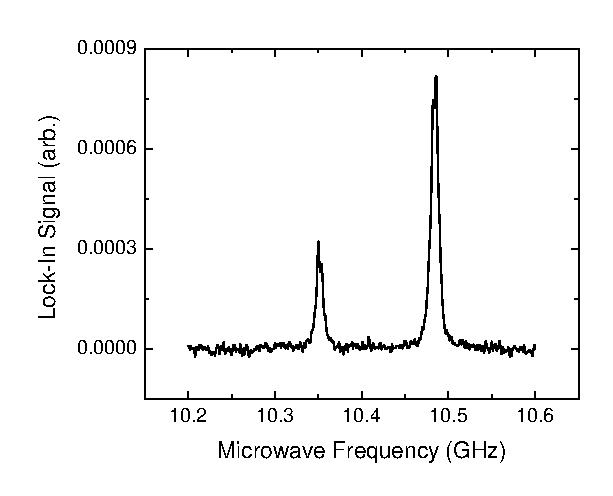
\includegraphics{p14-odmr}}
    \caption[Experimental ODMR\index{optically detected magnetic resonance (ODMR)} for SiC\index{silicon carbide (4H SiC)}]{\label{fig:SiCResults}
     The experimental ODMR results for 4H-SiC for a magnetic field strength of B=$370.78~\text{mT}$. Like the computational predictions, this plot also shows the the relation between microwave frequency absorption for a static magnetic field strength.}
 \end{figure}
 
\begin{figure}[H]
    \centerline{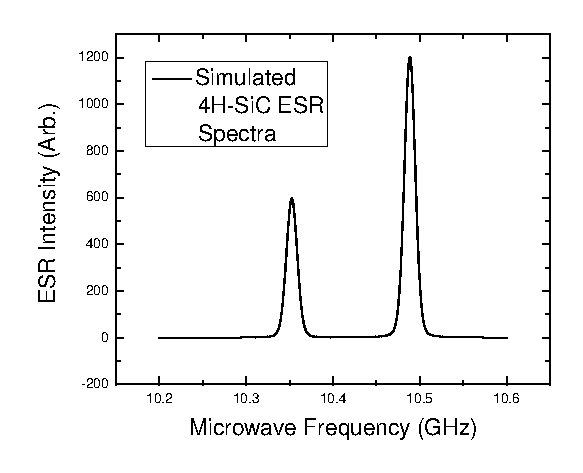
\includegraphics{p14-esr}}
    \caption[ESR\index{electron spin resonance (ESR)}\index{electron paramagnetic resonance (EPR)}\index{electron spin resonance (ESR)}\index{electron paramagnetic resonance (EPR)} Computational Model for SiC\index{silicon carbide (4H SiC)}]{\label{fig:SiCModelCorrected}
     The manually-corrected computational model for the ESR spectrum of 4H-SiC plotted for a magnetic field strength of B=$370.78~\text{mT}$. In this plot the first minor peak has been corrected to reflect unaccounted Hamiltonian parameters}
 \end{figure}

\section{Data Analysis}

The main expectation of the two different ESR\index{electron spin resonance (ESR)}\index{electron paramagnetic resonance (EPR)}\index{electron spin resonance (ESR)}\index{electron paramagnetic resonance (EPR)} methods is that both will produce spectral peaks at the same resonant microwave/magnetic field pairings. Moreover, it is also expected that the relative heights of each spectral peak are the same when compared between plots. The data presented in the previous sections corroborate at least the first of these two conditions. There is still is some differences between the two methods beyond these conditions. For example, the experimental ODMR\index{optically detected magnetic resonance (ODMR)} shows a higher noise-floor than the computational method. It's easier to predict cleaner spectras when the only uncertainty is that of machine precision and not environmental effects.

It is expected (and actually acceptable) that there will be some variations in the results obtained between the experiment and the theoretical models. The most notable difference between the two methods is seen in the width of each spectral peak within the plots. Though it is similar, there is a quantitative difference between the two plots. Theoretically the probability of transitioning between microwave-levels in the samples should reach a delta-function limit centered at the resonant frequency for that given field strength. However, in practice this does not happen due to inhomogeneities within the material itself. ESR\index{electron spin resonance (ESR)}\index{electron paramagnetic resonance (EPR)}\index{electron spin resonance (ESR)}\index{electron paramagnetic resonance (EPR)} peaks are instead shown to have finite widths in the magnetic-field domain. Though the experimental results are easily reproducible given the same parameters, different investigations may find different values of width depending on how the silicon carbide samples were produced. It is therefore not hard to explain why the computational predictions that were obtained for ESR\index{electron spin resonance (ESR)}\index{electron paramagnetic resonance (EPR)}\index{electron spin resonance (ESR)}\index{electron paramagnetic resonance (EPR)} do not always match the experimental results when there is such discrepancy among experimental procedures themselves. For our purposes a spectral line-width parameter was used to best match the experimental results that we obtained.

One of the major problems with modeling ESR spectra is that so many minor experimental conditions can fundamentally change the spin-system being studied and thus change what the resultant spectrum looks like when being modeled. As mentioned, computational models are only effective to the extent that the Hamiltonian for the system is understood. For the case of silicon carbide, there is still many details about the material that are not well understood --- or simply not known --- about the system. For example, there is still a lot of speculation and ignorance regarding the exact effect of the nuclear-spin interaction, the effects of the ODMR PL-mechanism, and the effects of the inhomegenous distribution of defects in the sample. To account for this, Figure \ref{fig:SiCModelCorrected} shows the data from Figure \ref{fig:SiCModel} except with the spectral peaks treated separately in the Hamiltonian such that the relative peak-heights can be adjusted appropriately to match the experimental results.

\section{Related Work}

\section{Conclusion}

The primary conclusion of this thesis is that though there are some differences between the two methods, the results show that computational ESR\index{electron spin resonance (ESR)}\index{electron paramagnetic resonance (EPR)}\index{electron spin resonance (ESR)}\index{electron paramagnetic resonance (EPR)} predictions match experimental results to the same extent that the underlying Hamiltonian for that particular system is understood. In other words: the level of precision that computational modeling can present is restricted by how much information is known about the Hamiltonian\index{spin Hamiltonian} for that given system. Furthermore, there will always be some ambiguity between ODMR\index{optically detected magnetic resonance (ODMR)} results and predictions due to practical considerations such as noise and ESR\index{electron spin resonance (ESR)}\index{electron paramagnetic resonance (EPR)}\index{electron spin resonance (ESR)}\index{electron paramagnetic resonance (EPR)} line-widths. Overall however, computational methods are good approximations of actual ESR\index{electron spin resonance (ESR)}\index{electron paramagnetic resonance (EPR)}\index{electron spin resonance (ESR)}\index{electron paramagnetic resonance (EPR)} results.


\begin{appendices}

\chapter{Electron Spin Coherence of Silicon Vacancies in Proton-Irradiated 4H-SiC}
\label{sec:appenda}

\chapter{Electron Spin Studies of Electron Irradiated SiC}
\label{sec:appendb}

\chapter{Optical Studies of Cadmium Telluride}
\label{sec:appendc}

\end{appendices}


% Make the bibliography.
% Enter your references in the BibTex file ''references.bib''
\bibliography{references}

% Make the index
\printindex

\end{document}
